\documentclass{standalone}
%outline around text
\usepackage[outline]{contour}
\contourlength{1.3pt}

%tikz
\usepackage{tikz}
\usetikzlibrary{knots, cd, calc}

\begin{document}

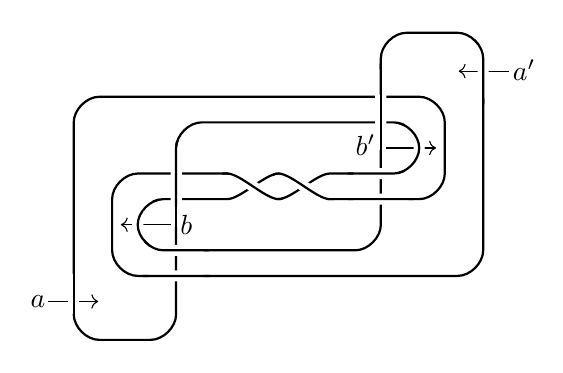
\begin{tikzpicture}[scale=0.65]
\clip (-4.9, -3.1) rectangle (5, 3.1);
\begin{knot}[clip width = 5, consider self intersections=true, ignore endpoint intersections = false,
%draft mode = crossings,
flip crossing/.list = {3, 6, 10, 7, 14}
]
\strand[thick] 
	(-4, -2.5) --
	(-4, 1.25) .. controls +(0, 0.25) and +(-0.25, 0) ..
	(-3.5, 1.75) --
	(2.75, 1.75) .. controls +(0.25, 0) and +(0, 0.25) ..
	(3.25, 1.25) -- 
	(3.25, 0.25) .. controls +(0, -0.25) and +(0.25, 0) ..
	(2.75, -0.25) -- 
	(1, -0.25) .. controls +(-0.25, 0) and +(0.25, 0) ..
	(0, 0.25) .. controls +(-0.25, 0) and +(0.25, 0) ..
	(-1, -0.25) --
	(-2.25, -0.25) .. controls +(-0.25, 0) and +(0, 0.25) ..
	(-2.75, -0.75) .. controls +(0, -0.25) and +(-0.25, 0) ..
	(-2.25, -1.25) --
	(1.5, -1.25) .. controls +(0.25, 0) and +(0, -0.25) ..
	(2, -0.75) --
	(2, 2.5) .. controls +(0, 0.25) and +(-0.25, 0) ..
	(2.5, 3) --
	(3.5, 3) .. controls +(0.25, 0) and +(0, 0.25) ..
	(4, 2.5) -- 
	(4, -1.25) .. controls +(0, -0.25) and +(0.25, 0) ..
	(3.5, -1.75) --
	(-2.75, -1.75) .. controls +(-0.25, 0) and +(0, -0.25) ..
	(-3.25, -1.25) -- 
	(-3.25, -0.25) .. controls +(0, 0.25) and +(-0.25, 0) ..
	(-2.75, 0.25) -- 
	(-1, 0.25) .. controls +(0.25, 0) and +(-0.25, 0) ..
	(0, -0.25) .. controls +(0.25, 0) and +(-0.25, 0) ..
	(1, 0.25) -- 
	(2.25, 0.25) .. controls +(0.25, 0) and +(0, -0.25) ..
	(2.75, 0.75) .. controls +(0, 0.25) and +(0.25, 0) ..
	(2.25, 1.25) -- 
	(-1.5, 1.25) .. controls +(-0.25, 0) and +(0, 0.25) ..
	(-2, 0.75) --
	(-2, -2.5) .. controls +(0, -0.25) and +(0.25, 0) ..
	(-2.5, -3) --
	(-3.5, -3) .. controls +(-0.25, 0) and +(0, -0.25) ..
	(-4, -2.5);
	
\strand[->] (-4.5, -2.25) -- (-3.5, -2.25);
\strand[->] (4.5, 2.25) -- (3.5, 2.25);
\strand[->] (-2.1, -0.75) -- (-3.1, -0.75);
\strand[->] (2.1, 0.75) -- (3.1, 0.75);
\end{knot}
\node at (-4.7, -2.25) {$a$};
\node at (4.8, 2.28) {$a'$};
\node at (-1.8, -0.75) {$b$};
\node at (1.7, 0.8) {$b'$};
\end{tikzpicture}

\end{document}